% Provenance (never printed): see sources/outline_sources.md (Year 1: the general
% circulation of the atmosphere, Hadley, Ferrel and polar cells, the ITCZ, Walker cells,
% jet streams, the geostrophic wind, depressions and anticyclones). Exercise and problem
% values in the Book 3 scratch calculator calc/ch28.py; figures from
% figdata/bachelor-1/angular_momentum_wind.py, weather_map.py (an invented map) and
% general_circulation.py (NCEP-NCAR Reanalysis 1, long-term means 1991-2020, datasets
% bachelor-1-ncep-{uwnd-p,vwnd-p,uwnd-sfc,slp,prate-monthly}).
% Physics owns the Coriolis force and the hydrostatic relation (recalled). Book 1 (g8) gave
% the global winds, the convection cell, depressions and anticyclones, isobars and the
% rotation of the wind around them, in words: re-founded here with forces and data.
% ENSO and the monsoons are the Year 2 volume's; the thermal wind the Year 3 volume's.
\chapter{الدوران العام للغلاف الجوي}\label{ch:b1:atmospheric-circulation}

ارتادت السفن الشراعية التي عبرت من أوروبا وأفريقيا إلى الأمريكتين على \omterm{def:b1:atmospheric-circulation:winds}{الرياح التجارية}، وهي شرقيّات ثابتة في المدارات. وأقرب إلى خطّ الاستواء، على نحو خمس درجات منه، تضعف الرياح نفسها في نطاق السكون والأمطار المتقطّعة الذي سمّاه البحّارة «الهدوء الاستوائي». وعلى ارتفاع نحو تسعة كيلومترات فوق الاثنين، يمكن لأنهار هوائية ضيّقة تُسمّى تيّارات النفّاثة أن تهبّ بأكثر من \qty{440}{km/h}. يشرح هذا الفصل الثلاثة: لماذا ينتهي الهواء المتحرّك فوق كوكب دوّار إلى الهبوب على طول الخطوط المتساوية الضغط لا عبرها، وكيف يدفع فائض المدارات خليّة قلب ضخمة على كل جانب من خطّ الاستواء، ولماذا يتحوّل الهواء الذي يغادر خطّ الاستواء في الأعلى إلى تيّار نفّاث غربي.
% ledger: nos:trade-winds, nos:doldrums, noaajs:jet

\begin{omfigure}
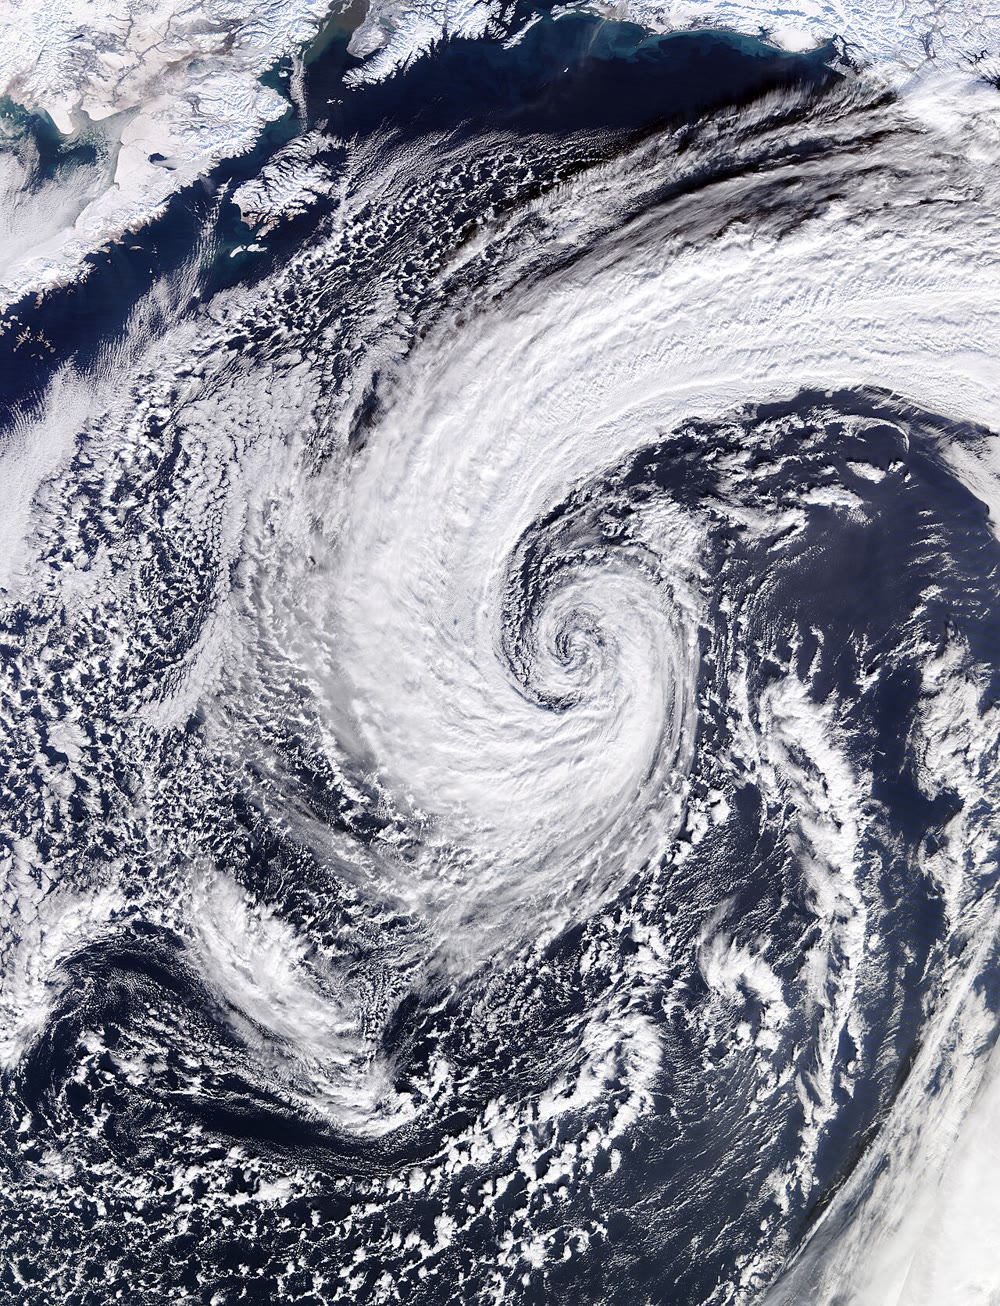
\includegraphics[width=0.5\linewidth]{images/book3/b1-alaska-low.jpg}

{\small منخفض جوّي خارج المدارات فوق خليج ألاسكا في 28 يناير 2018، مُرصد بجهاز MODIS من المدار؛ الساحل المكسوّ بالثلج لألاسكا في أعلى اليسار، والشمال تقريبًا إلى الأعلى. تلتفّ نطاقات السحب عكس عقارب الساعة نحو المركز، كما يفعل هواء المنخفض في نصف الكرة الشمالي. (NASA, MODIS/LANCE, ملك عام، عبر Wikimedia Commons.)}
\label{fig:b1:atmospheric-circulation:alaska}
\end{omfigure}
% ledger: commons:alaska-low, nws:cyclone

\begin{recall}
تعطي كتب الفيزياء العلاقة الهيدروستاتيكية وقوة كوريوليس: في إطار يدور بسرعة زاوية $\vec\Omega$، يشعر جسم كتلته $m$ يتحرّك بسرعة $\vec v$ بالنسبة إلى الإطار بقوة وهمية $-2m\,\vec\Omega\times\vec v$، عمودية على حركته. وللأرض، $\Omega = 2\pi/T_\star$ مع اليوم النجمي $T_\star = \qty{23.9345}{h}$، أي $\Omega = \qty{7.292e-5}{rad.s^{-1}}$. وصف الكتاب~1 الرياح الكوكبية (\omterm{def:b1:atmospheric-circulation:winds}{الرياح التجارية}، \omterm{def:b1:atmospheric-circulation:winds}{والرياح الغربية}، والشرقيات القطبية)، وخليّة الحمل، والمنخفضات والمرتفعات الجوّية، وخطوط الضغط المتساوي في الخريطة الجوّية، ودوران الرياح حول المراكز. \Cref{ch:b1:fluid-envelopes-structure} أعطى \omterm{def:b1:fluid-envelopes-structure:standard-atmosphere}{الغلاف الجوي المعياري} \omterm{def:b1:fluid-envelopes-structure:lapse-rate}{ومعدّل الانخفاض الأديباتي الجاف}، و\cref{ch:b1:radiation-heat-transport} النقل الحراري نحو القطبين الذي تحمله الدورة.
% ledger: earth:Trot, nws:coriolis
\end{recall}

\section{القوى المؤثّرة في الهواء المتحرّك}\label{sec:b1:atmospheric-circulation:forces}

يُدفع جزيء الهواء بضغط الهواء المحيط به، ويُجذب بالجاذبية، ويُبطّأ بالاحتكاك قرب الأرض، وينحرف، عند رصده من الأرض الدوّارة، بقوة كوريوليس. وتتعادل الجاذبية وقوة الضغط الرأسية تقريبًا تمامًا: وهذه هي العلاقة الهيدروستاتيكية. والطقس تصنعه القوى التي تبقى في الأفقي.

\begin{definition}[قوة تدرّج الضغط]\label{def:b1:atmospheric-circulation:pgf}
\emph{قوة تدرّج الضغط}\index{قوة تدرّج الضغط} هي القوة الصافية التي يؤثّر بها ضغط المائع المحيط في جزء من المائع. ولكل وحدة كتلة تكون $-(1/\rho)\nabla p$، حيث $\rho$ الكثافة و$\nabla p$ تدرّج الضغط: تتّجه من الضغط المرتفع نحو المنخفض، عبر الخطوط المتساوية الضغط.
\end{definition}
% ledger: nws:geostrophic

\begin{proposition}[قوة تدرّج الضغط]\label{prop:b1:atmospheric-circulation:pgf}
على جزء حجمه $\mathrm dV$ وكثافته $\rho$، يؤثّر ضغط المائع المحيط بقوة $-\nabla p\,\mathrm dV$، أي تسارع $-(1/\rho)\nabla p$.
\end{proposition}

\begin{proof}
خذ صندوقًا صغيرًا أضلاعه $\mathrm dx$ و$\mathrm dy$ و$\mathrm dz$ على المحاور. على وجهه عند $x$، يدفع الضغط في اتجاه $+x$ بالقوة $p(x)\,\mathrm dy\,\mathrm dz$؛ وعلى وجهه عند $x + \mathrm dx$، في اتجاه $-x$ بالقوة $p(x + \mathrm dx)\,\mathrm dy\,\mathrm dz$. والقوة الصافية على طول $x$ هي $[p(x) - p(x + \mathrm dx)]\,\mathrm dy\,\mathrm dz = -(\partial p/\partial
x)\,\mathrm dV$، وكذلك على طول $y$ و$z$. والمجموع هو $-\nabla p\,
\mathrm dV$؛ وبقسمته على الكتلة $\rho\,\mathrm dV$ نحصل على التسارع.
\end{proof}

لا يولّد الضغط المنتظم قوّة صافية: لا تدفع إلا الفروق. وعلى الخريطة الجوّية يُقرأ التدرّج الأفقي من الخطوط المتساوية الضغط: قيمته هي فرق الضغط بين خطّين متتاليين مقسومًا على بعدهما. فلخطوط تفصل بينها \qty{4}{hPa} وتبعد \qty{400}{km} عند مستوى البحر، حيث $\rho \approx \qty{1.225}{kg.m^{-3}}$، يكون التسارع $400/(1.225 \times \num{4e5}) = \qty{8.2e-4}{m.s^{-2}}$، أي أقلّ من جزء من عشرة آلاف من $g$، ومع ذلك يكفي لأن يبلغ الهواء من السكون \qty{10}{m/s} في ثلاث ساعات ونصف.
% ledger: ussa76:sea-level

يشعر الهواء بقوة كوريوليس لأنه يُرصد من أرض دوّارة. وجزؤه الأفقي يعتمد على خطّ العرض عبر عدد واحد.

\begin{definition}[معامل كوريوليس]\label{def:b1:atmospheric-circulation:coriolis-parameter}
\emph{معامل كوريوليس}\index{معامل كوريوليس} عند خطّ العرض $\varphi$ هو
$f = 2\Omega\sin\varphi$، حيث $\Omega$ هي السرعة الزاوية للأرض. وهو موجب في نصف الكرة الشمالي، وسالب في الجنوبي، ومعدوم عند خطّ الاستواء، وأكبر ما يكون عند القطبين، $2\Omega = \qty{1.458e-4}{s^{-1}}$.
\end{definition}
% ledger: earth:Trot

\begin{proposition}[التسارع الأفقي لكوريوليس]\label{prop:b1:atmospheric-circulation:coriolis}
بالنسبة إلى ريح أفقية $\vec v$ عند خطّ العرض $\varphi$، يكون الجزء الأفقي من تسارع كوريوليس $-f\,\vec k\times\vec v$، حيث $\vec k$ الاتجاه الرأسي الصاعد: مقداره $|f|\,|\vec v|$، ويتّجه عموديًّا على الريح، إلى يمينها في نصف الكرة الشمالي، وإلى يسارها في الجنوبي.
\end{proposition}

\begin{proof}
استخدم محاور محلّية: $x$ شرقًا، و$y$ شمالًا، و$z$ صعودًا. يقع متّجه دوران الأرض في مستوى الزوال، عند الزاوية $\varphi$ فوق الأفق الشمالي: $\vec\Omega =
\Omega(0, \cos\varphi, \sin\varphi)$. وبالنسبة إلى $\vec v = (u, v, 0)$،
\[
  \vec\Omega\times\vec v = \Omega\,(-v\sin\varphi,\ u\sin\varphi,\ -u\cos\varphi),
  \qquad -2\vec\Omega\times\vec v = (f v,\ -f u,\ 2\Omega u\cos\varphi).
\]
بما أن $\vec k\times\vec v = (-v, u, 0)$، فالجزء الأفقي $(fv, -fu)$ هو
$-f\,\vec k\times\vec v$. والمتّجه $\vec k\times\vec v$ هو $\vec v$ مُدارًا بمقدار \ang{90} عكس عقارب الساعة عند النظر من الأعلى؛ ومعكوسه هو $\vec v$ مُدارًا باتجاه عقارب الساعة، إلى اليمين حين $f > 0$، وإلى اليسار حين $f < 0$.
\end{proof}
% ledger: earth:Trot

الجزء الرأسي، $2\Omega u\cos\varphi$، يبلغ على الأكثر \qty{1.5e-3}{m.s^{-2}} لرياح قدرها \qty{10}{m/s}، أي نحو \num{1.5e-4} من $g$: والتوازن الهيدروستاتيكي يمتصّه. أمّا الجزء الأفقي، مهما كان صغيرًا، فلا منافس له في الغلاف الجوي الحرّ فوق طبقة الاحتكاك، وعلى مدى ساعات يشكّل كل ريح.

وقرب الأرض يحتكّ الهواء أيضًا بالسطح. وفي الكيلومتر الأدنى، طبقة الاحتكاك كما يسمّيها علماء الأرصاد الجوية، يغيّر الاحتكاك سرعة الريح واتجاهها معًا؛ إذ تحمل الدوّامات المضطربة سحب السطح إلى الأعلى، وتعمل القوة تقريبًا عكس الريح وتزداد معها. وفوق ذلك، في الغلاف الجوي الحرّ، يكون الاحتكاك ضئيلًا.
% ledger: nws:friction-layer

\section{الرياح الجيوستروفية}\label{sec:b1:atmospheric-circulation:geostrophic}

\begin{definition}[التوازن الجيوستروفي، والريح الجيوستروفية]\label{def:b1:atmospheric-circulation:geostrophic}
يكون التدفّق الأفقي في \emph{توازن جيوستروفي}\index{توازن جيوستروفي} حين تلغي قوته \omterm{def:b1:atmospheric-circulation:pgf}{قوة تدرّج الضغط} وقوة كوريوليس بعضهما. و\emph{الريح الجيوستروفية}\index{الريح الجيوستروفية} $\vec v_g$ هي الريح التي تحقّق هذا التوازن لحقل ضغط معيّن: $-(1/\rho)\nabla p - f\,\vec k\times\vec v_g = \vec 0$.
\end{definition}
% ledger: nws:geostrophic

\begin{theorem}[الريح الجيوستروفية]\label{thm:b1:atmospheric-circulation:geostrophic}
بعيدًا عن خطّ الاستواء،
\[
  \vec v_g = \frac{1}{\rho f}\,\vec k\times\nabla p, \qquad
  |\vec v_g| = \frac{|\nabla p|}{\rho\,|f|} .
\]
تهبّ \omterm{def:b1:atmospheric-circulation:geostrophic}{الريح الجيوستروفية} على طول الخطوط المتساوية الضغط، وتكون أسرع حيث تتقارب. وفي نصف الكرة الشمالي تُبقي الضغط المنخفض على يسارها؛ وفي نصف الكرة الجنوبي، على يمينها.
\end{theorem}

\begin{proof}
بالنسبة إلى متّجه أفقي $\vec w$، يكون $\vec k\times(\vec k\times\vec w) = -\vec w$.
بتطبيق $\vec k\times$ على التوازن $f\,\vec k\times\vec v_g = -(1/\rho)\nabla p$ نحصل على $-f\vec v_g = -(1/\rho)\,\vec k\times\nabla p$، ومنه الصيغة، الصالحة حيث $f \neq 0$. وبما أن $\vec k\times\nabla p$ عمودي على $\nabla p$، فالريح عمودية على التدرّج، أي على طول الخطوط المتساوية الضغط؛ ومقدارها $|\nabla
p|/(\rho|f|)$. والمتّجه $\vec k\times\nabla p$ هو التدرّج مُدارًا بمقدار \ang{90} عكس عقارب الساعة. وبالسير في اتجاهه، يقع التدرّج، الذي يشير إلى الضغط المرتفع، على اليمين، فيقع الضغط المنخفض على اليسار؛ وحين $f > 0$ تكون للريح اتجاه $\vec k\times\nabla p$، وحين $f < 0$ يكون اتجاهها المعاكس.
\end{proof}

\begin{example}[ريح تُقرأ من الخطوط المتساوية الضغط]\label{ex:b1:atmospheric-circulation:geostrophic}
عند \ang{50} شمالًا، $f = 2 \times \num{7.292e-5} \times \sin\ang{50} = \qty{1.117e-4}{s^{-1}}$.
خطوط تفصل بينها \qty{4}{hPa} وتبعد \qty{400}{km} تعطي $|\nabla p| = 400/\num{4e5} =
\qty{1.0e-3}{Pa.m^{-1}}$ و، مع $\rho = \qty{1.225}{kg.m^{-3}}$، ريحًا جيوستروفية قدرها $\num{1.0e-3}/(1.225 \times \num{1.117e-4}) = \qty{7.3}{m/s}$. والتباعد نفسه عند \ang{20} شمالًا، حيث $f$ أقلّ من نصف قيمته، يعطي \qty{16.4}{m/s}.
\end{example}
% ledger: earth:Trot, ussa76:sea-level

التوازن ليس لحظيًّا. فالهواء الذي تحرّكه تدرّج ضغط يدور تحت قوة كوريوليس بمعدّل $f$، أي مرّة كل $2\pi/f$، نحو ست عشرة ساعة عند \ang{50} شمالًا؛ والأنماط التي تدوم أكثر من بضع ساعات، وتكون أكبر من بضع مئات الكيلومترات، تقترب من الجيوستروفية. وقرب خطّ الاستواء تميل $f$ إلى الصفر، فتنهار الصيغة، ولا تكون رياح المدارات العميقة جيوستروفية.

\begin{omfigure}
\begin{tikzpicture}[>={Stealth[length=2.2mm]}, font=\scriptsize]
  % left panel: geostrophic balance
  \begin{scope}
    \draw[isobar] (-2.4,1.2) -- (2.4,1.2) node[right] {\qty{996}{hPa}};
    \draw[isobar] (-2.4,0) -- (2.4,0) node[right] {\qty{1000}{hPa}};
    \draw[isobar] (-2.4,-1.2) -- (2.4,-1.2) node[right] {\qty{1004}{hPa}};
    \node[pressure low] at (0,2.0) {L};
    \node[pressure high] at (0,-2.0) {H};
    \fill (0,0) circle (1.6pt);
    \draw[->, very thick, omThm] (0,0) -- (0,1.0);
    \node[omThm, anchor=east] at (-0.08,0.6) {تدرّج الضغط};
    \draw[->, very thick, omDef] (0,0) -- (0,-1.0);
    \node[omDef, anchor=east] at (-0.08,-0.6) {كوريوليس};
    \draw[->, line width=1.6pt, black] (0,0) -- (1.9,0) node[above, pos=0.75] {الريح $\vec v_g$};
    \node[anchor=north] at (0,-2.4) {بلا احتكاك: جيوستروفية};
  \end{scope}
  % right panel: with friction (alpha = 25 deg, V = Vg cos alpha)
  \begin{scope}[xshift=7.4cm]
    \draw[isobar] (-2.4,1.2) -- (2.4,1.2) node[right] {\qty{996}{hPa}};
    \draw[isobar] (-2.4,0) -- (2.4,0) node[right] {\qty{1000}{hPa}};
    \draw[isobar] (-2.4,-1.2) -- (2.4,-1.2) node[right] {\qty{1004}{hPa}};
    \node[pressure low] at (0,2.0) {L};
    \node[pressure high] at (0,-2.0) {H};
    \fill (0,0) circle (1.6pt);
    \draw[->, very thick, omThm] (0,0) -- (0,1.0);
    \node[omThm, anchor=east] at (-0.08,0.6) {تدرّج الضغط};
    \draw[->, very thick, omDef] (0,0) -- ({1.0*cos(25)*sin(25)},{-1.0*cos(25)*cos(25)});
    \node[omDef, anchor=west] at (0.42,-0.62) {كوريوليس};
    \draw[->, very thick, omMeth] (0,0) -- ({-1.0*sin(25)*cos(25)},{-1.0*sin(25)*sin(25)})
      node[below left, inner sep=1pt] {الاحتكاك};
    \draw[->, line width=1.6pt, black] (0,0) -- ({1.9*cos(25)*cos(25)},{1.9*cos(25)*sin(25)})
      node[above, inner sep=2pt] {الريح $\vec v$};
    \draw[black!50, dashed] (0,0) -- (1.9,0);
    \draw[black!60] (1.0,0) arc[start angle=0, end angle=25, radius=1.0];
    \node[black!70] at (1.22,0.22) {$\alpha$};
    \node[anchor=north] at (0,-2.4) {مع الاحتكاك: أبطأ، وعبر الخطوط المتساوية الضغط};
  \end{scope}
\end{tikzpicture}

{\small قوى على جزء من الهواء في نصف الكرة الشمالي، والضغط المنخفض شمالًا. يسارًا: في الغلاف الجوي الحرّ تلغي \omterm{def:b1:atmospheric-circulation:pgf}{قوة تدرّج الضغط} (أحمر) وقوة كوريوليس (أزرق) بعضهما، فتهبّ الريح على طول الخطوط المتساوية الضغط والمنخفض على يسارها. يمينًا: قرب الأرض يعمل الاحتكاك (أخضر) عكس الريح؛ ولا تتوازن القوى الثلاث إلا إذا كانت الريح أبطأ وانحرفت بزاوية $\alpha$ نحو المنخفض (مرسومة من أجل $\alpha = \ang{25}$ وسحب \cref{prop:b1:atmospheric-circulation:friction}).}
\label{fig:b1:atmospheric-circulation:balance}
\end{omfigure}

\begin{proposition}[الاحتكاك يُدير الريح نحو الضغط المنخفض]\label{prop:b1:atmospheric-circulation:friction}
لنفترض أن ريحًا أفقية ثابتة $\vec v$ تؤثّر فيها \omterm{def:b1:atmospheric-circulation:pgf}{قوة تدرّج الضغط}، وقوة كوريوليس، وقوة احتكاك $-\vec v/\tau$، حيث $\tau > 0$، عند خطّ عرض حيث $f > 0$. عندئذٍ تعبر الريح الخطوط المتساوية الضغط نحو الضغط المنخفض بزاوية $\alpha$ حيث $\tan\alpha = 1/(f\tau)$، وسرعتها $|\vec v| =
|\vec v_g|\cos\alpha$، أدنى من \omterm{def:b1:atmospheric-circulation:geostrophic}{الريح الجيوستروفية}.
\end{proposition}

\begin{proof}
ليكن $V = |\vec v|$، و$\hat v$ متّجه الوحدة على طول الريح، و$\hat n$ متّجه الوحدة العمودي عليها، إلى يسارها. التوازن هو $-(1/\rho)\nabla p - f\,
\vec k\times\vec v - \vec v/\tau = \vec 0$، و$\vec k\times\vec v = V\hat n$.
على طول $\hat v$: $-(1/\rho)\,\nabla p\cdot\hat v = V/\tau > 0$، فللريح مركّبة في اتجاه التدرّج نحو الضغط المنخفض. وعلى طول $\hat n$:
$-(1/\rho)\,\nabla p\cdot\hat n = fV$. \omterm{def:b1:atmospheric-circulation:pgf}{وقوة تدرّج الضغط}، ومقدارها $P =
|\nabla p|/\rho = f|\vec v_g|$، لها إذن مركّبتان $V/\tau$ على طول الريح و$fV$ عبرها: فهي تصنع مع الريح الزاوية $\beta$ حيث $\tan\beta =
1/(f\tau)$، و$P^2 = V^2(f^2 + 1/\tau^2)$. والخطوط المتساوية الضغط عمودية على التدرّج، فالريح تعبرها بزاوية $\alpha = \beta$، و$V = P/\sqrt{f^2 +
1/\tau^2} = (P/f)\cos\alpha = |\vec v_g|\cos\alpha$.
\end{proof}

سطح أخشن يعني سحبًا أقوى، و$\tau$ أقصر، وزاوية أكبر: فتعبر الريح الخطوط المتساوية الضغط بانحدار أشدّ فوق اليابسة منه فوق البحر. والاحتكاك الحقيقي ليس خطّيًّا تمامًا في الريح، لكن الخلاصة، أي أنها أبطأ وتنحرف نحو المنخفض، عامّة.

\begin{remark}[الريح التدرّجية]\label{rem:b1:atmospheric-circulation:gradient}
حول مركز تكون الخطوط المتساوية الضغط منحنية، والهواء الذي يتبعها يتسارع نحو مركز التقوّس، أي $V^2/r$ لدائرة نصف قطرها $r$. وحول منخفض في نصف الكرة الشمالي، يجب إذن أن تتجاوز \omterm{def:b1:atmospheric-circulation:pgf}{قوة تدرّج الضغط} قوة كوريوليس: $fV + V^2/r = f|\vec v_g|$، وتكون الريح، المسمّاة الريح التدرّجية، أضعف من الجيوستروفية. وحول مرتفع، يجب أن تتجاوز قوة كوريوليس \omterm{def:b1:atmospheric-circulation:pgf}{قوة تدرّج الضغط}، $fV - V^2/r = f|\vec v_g|$: الريح أقوى، لكن المعادلة لا تملك حلًّا إلا إذا كان $|\vec v_g| \leq fr/4$، وهذا يمنع تدرّجات ضغط قوية قرب مركز \omterm{def:b1:atmospheric-circulation:cyclone}{المرتفع الجوّي} (\cref{exo:b1:atmospheric-circulation:10}).
\end{remark}

\section{المنخفضات والمرتفعات الجوّية}\label{sec:b1:atmospheric-circulation:cyclones}

\begin{definition}[المنخفض الجوّي والمرتفع الجوّي]\label{def:b1:atmospheric-circulation:cyclone}
\emph{المنخفض الجوّي}\index{المنخفض الجوّي} دوران واسع النطاق للرياح حول مركز ضغط منخفض، أي منخفض جوّي؛ و\emph{المرتفع الجوّي}\index{المرتفع الجوّي} دوران حول مركز ضغط مرتفع. يدور المنخفض الجوّي عكس عقارب الساعة في نصف الكرة الشمالي، وفي عقاربها في الجنوبي؛ والمرتفع الجوّي بالعكس.
\end{definition}
% ledger: nws:cyclone

تنبع اتجاهات الدوران من \cref{thm:b1:atmospheric-circulation:geostrophic}: في نصف الكرة الشمالي، تدور ريح تُبقي المنخفض على يسارها حوله عكس عقارب الساعة، وحول المرتفع في عقاربها. وترى من الفضاء سحب المنخفض تُظهر الدوران (الصورة في مطلع الفصل)؛ وفي نصف الكرة الجنوبي تكون الحلزونات صورًا معكوسة.
% ledger: nws:cyclone, commons:alaska-low

\begin{history}[قانون بايس بالوت، 1857]
في 1857 صاغ عالم الأرصاد الهولندي C.~H.~D. Buys Ballot قاعدة وجدتها المشاهدات: في نصف الكرة الشمالي، من يقف ظهره إلى الريح يكون الضغط المنخفض على يساره والمرتفع على يمينه؛ وفي نصف الكرة الجنوبي، العكس. ولم يكن يعرف أن عالم الأرصاد الأمريكي William Ferrel كان قد استنتجها من النظرية، فاعترف لاحقًا بأولوية Ferrel. \omterm{def:b1:atmospheric-circulation:geostrophic}{والريح الجيوستروفية} هي القانون في المعادلات.
\end{history}
% ledger: skybrary:buys-ballot

ويضيف الاحتكاك التواءً مهمًّا. قرب الأرض تعبر الريح الخطوط المتساوية الضغط نحو الضغط المنخفض (\cref{prop:b1:atmospheric-circulation:friction}): فحول المنخفض يلتفّ الهواء نحو الداخل، ويتقارب قرب الأرض، ويجب أن يصعد. والهواء الصاعد يتمدّد ويبرد \omterm{def:b1:fluid-envelopes-structure:lapse-rate}{بمعدّل الانخفاض الأديباتي الجاف} (\cref{ch:b1:fluid-envelopes-structure})، وحين يبلغ التشبّع يتكثّف بخاره: فالمنخفضات تجلب السحب والمطر. وحول \omterm{def:b1:atmospheric-circulation:cyclone}{المرتفع الجوّي} ينتشر هواء السطح نحو الخارج؛ فيهبط هواء من الأعلى ليحلّ محلّه، ويسخن بالضغط وتتبخّر سحبه: فالمرتفعات الجوّية تجلب طقسًا مستقرًّا، غالبًا صافيًا.
% ledger: nws:dalr

الخريطة أدناه مثال مخترَع، محسوب لا مرصود: منخفض عمقه \qty{28}{hPa} ومرتفع ارتفاعه \qty{20}{hPa} على خلفية \qty{1013}{hPa}، مركزهما قرب \ang{50} شمالًا. وعند كل محطة يبيّن ريشُ \omterm{def:b1:atmospheric-circulation:geostrophic}{الريح الجيوستروفية} المحسوبة من الخريطة ب\cref{thm:b1:atmospheric-circulation:geostrophic}.

\begin{omfigure}
\pgfplotstableread{figdata/out/bachelor-1-weather_map-stations.dat}\wmstations
\pgfplotstableread{figdata/out/bachelor-1-weather_map-labels.dat}\wmlabels
\begin{tikzpicture}
\begin{axis}[x=0.0038cm, y=0.0038cm, disabledatascaling, anchor=origin,
  xmin=-1800, xmax=1800, ymin=-1200, ymax=1200, xtick=\empty, ytick=\empty,
  axis background/.style={fill=blue!4}, clip=true]
% figdata/bachelor-1/weather_map.py (invented pressure field); ledger: earth:Trot, ussa76:sea-level
\addplot[isobar, unbounded coords=jump] table[x=x, y=y] {figdata/out/bachelor-1-weather_map-isobars.dat};
\addplot[black!45, dashed, domain=-1800:1800] {0};
\addplot[only marks, mark=none, nodes near coords, point meta=explicit symbolic,
  nodes near coords style={font=\tiny, fill=blue!4, inner sep=0.5pt, anchor=center}]
  table[x=x, y=y, meta=p] {\wmlabels};
\node[pressure low] at (axis cs:-500,150) {L};
\node[pressure high] at (axis cs:1050,-250) {H};
\node[font=\tiny, anchor=south west, black!60] at (axis cs:-1790,5) {\ang{50} شمالًا};
\end{axis}
\pgfplotstablegetrowsof{\wmstations}
\pgfmathtruncatemacro{\wmlast}{\pgfplotsretval-1}
\begin{scope}
\clip (-6.84,-4.56) rectangle (6.84,4.56);
\foreach \i in {0,...,\wmlast}{
  \pgfplotstablegetelem{\i}{x}\of\wmstations \let\wx\pgfplotsretval
  \pgfplotstablegetelem{\i}{y}\of\wmstations \let\wy\pgfplotsretval
  \pgfplotstablegetelem{\i}{speed_kn}\of\wmstations \let\ws\pgfplotsretval
  \pgfplotstablegetelem{\i}{from_deg}\of\wmstations \let\wd\pgfplotsretval
  \pic[transform shape] at ({\wx*0.0038},{\wy*0.0038}) {windbarb={\ws}{\wd}};
}
\end{scope}
\pic[transform shape] at (-6.5,-4.0) {scalebar={1.9}{\qty{500}{km}}};
\pic[scale=0.7, transform shape] at (-6.45,3.2) {northarrow};
\end{tikzpicture}

{\small خريطة ضغط مخترعة على مستوى البحر قرب \ang{50} شمالًا (الخطوط المتساوية الضغط كل \qty{4}{hPa}؛ الضغط المركزي \qty{986}{hPa} و\qty{1033}{hPa}). يشير كل ريش إلى \omterm{def:b1:atmospheric-circulation:geostrophic}{الريح الجيوستروفية} عند محطته، والعصا نحو المكان الذي تأتي منه الريح؛ الريش الكامل \qty{10}{kn}، والنصف \qty{5}{kn}، والعلم \qty{50}{kn} (\qty{1}{kn} = \qty{0.514}{m/s}). تلتفّ الرياح عكس عقارب الساعة حول المنخفض وفي عقاربها حول المرتفع، وتكون أقوى حيث تتزاحم الخطوط بينهما، فتبلغ \qty{36}{m/s}.}
\label{fig:b1:atmospheric-circulation:weather-map}
\end{omfigure}
% ledger: earth:Trot, ussa76:sea-level (computed in figdata/bachelor-1/weather_map.py)

\section{دورة الخلايا الثلاث}\label{sec:b1:atmospheric-circulation:cells}

متوسطةً حول الكرة وعلى مدى سنوات كثيرة، تكون الرياح التي تهبّ شمالًا أو جنوبًا ضعيفة، بضعة أمتار في الثانية على الأكثر، لكنها تحمل كتلة كبيرة من الهواء. ويُرى نمطها بأوضح صورة في الكتلة التي تتدفّق بين خطّ الاستواء والقطبين.

\begin{definition}[دالّة التيّار الميريدية المتوسطة]\label{def:b1:atmospheric-circulation:streamfunction}
\emph{دالّة التيّار الميريدية المتوسطة}\index{دالّة التيّار الميريدية المتوسطة}
$\psi(p, \varphi)$ هي كتلة الهواء في الثانية التي تعبر خطّ العرض
$\varphi$ شمالًا فوق مستوى الضغط $p$، في المتوسط النطاقي والزمني:
\[
  \psi(p, \varphi) = \frac{2\pi a_\oplus\cos\varphi}{g}\int_0^p [v]\,\mathrm dp' ,
\]
حيث $[v]$ الريح الشمالية المتوسطة حول الموازي. وتُقاس بوحدة \unit{kg.s^{-1}}.
\end{definition}

بما أن $\mathrm dp' = -\rho g\,\mathrm dz$ بالعلاقة الهيدروستاتيكية، فإن $2\pi a_\oplus
\cos\varphi\,[v]\,\mathrm dp'/g$ هو تدفّق الكتلة عبر حلقة من الموازي. فالهواء الذي يعبر الموازي فوق $p$ يجب أن يعبره في الاتجاه الآخر تحت $p$، لأن الكتلة لا تتراكم: تتلاشى $\psi$ عند الأرض وفي القمّة، وخطوط القيمة المتساوية فيها هي مسارات الدورة المتوسطة. والخليّة التي فيها $\psi > 0$ تدور في اتجاه عقارب الساعة حين يكون القطب الشمالي على اليمين: شمالًا في الأعلى، وجنوبًا في الأسفل.

\begin{omfigure}
\begin{tikzpicture}
\begin{groupplot}[group style={group size=1 by 2, vertical sep=1.3cm},
  width=0.82\linewidth, height=4.6cm, view={0}{90}, xmin=-70, xmax=70, ymin=100,
  ymax=1000, y dir=reverse, ytick={200,400,600,800,1000}, xtick={-60,-40,...,60},
  tick label style={font=\scriptsize}, label style={font=\small},
  ylabel={الضغط (\unit{hPa})},
  colormap={omdiv}{rgb255=(33,102,172) rgb255=(146,197,222) rgb255=(247,247,247)
    rgb255=(244,165,130) rgb255=(178,24,43)},
  point meta min=-22, point meta max=22, colorbar,
  colorbar style={width=0.25cm, y dir=normal, ytick={-20,-10,0,10,20}, tick label style={font=\scriptsize},
    ylabel={$\psi$ (\qty{e10}{kg.s^{-1}})}, ylabel style={font=\scriptsize}},
  axis on top, grid=none]
\nextgroupplot[title={ديسمبر--فبراير}, title style={font=\small}]
% figdata/bachelor-1/general_circulation.py; ledger: data:b3-ncep-circ, psl:ncep-r1
\addplot3[surf, shader=interp, mesh/ordering=x varies, mesh/cols=73]
  table[x=lat, y=p, z=psi] {figdata/out/bachelor-1-general_circulation-psi-djf.dat};
\addplot3[black, line width=0.5pt, unbounded coords=jump]
  table[x=lat, y=p, z expr=40] {figdata/out/bachelor-1-general_circulation-psi0-djf.dat};
\nextgroupplot[title={يونيو--أغسطس}, title style={font=\small}, xlabel={خطّ العرض (\unit{\degree})}]
\addplot3[surf, shader=interp, mesh/ordering=x varies, mesh/cols=73]
  table[x=lat, y=p, z=psi] {figdata/out/bachelor-1-general_circulation-psi-jja.dat};
\addplot3[black, line width=0.5pt, unbounded coords=jump]
  table[x=lat, y=p, z expr=40] {figdata/out/bachelor-1-general_circulation-psi0-jja.dat};
\end{groupplot}
\end{tikzpicture}

{\small \omterm{def:b1:atmospheric-circulation:streamfunction}{دالّة التيّار الميريدية المتوسطة} في الشتاء الشمالي (أعلى) والصيف الشمالي (أسفل)، من الريح الشمالية المتوسطة حول الموازي للتحليل المُعاد NCEP-NCAR Reanalysis~1، متوسطات 1991--2020 (البيانات من NOAA PSL). أحمر: خلايا تدور في اتجاه عقارب الساعة في هذا المنظور (صاعدة على جانبها الجنوبي)، أزرق: عكس عقارب الساعة؛ أسود: خطوط الصفر التي تفصل الخلايا. تحيط \omterm{def:b1:atmospheric-circulation:cells}{خليّة هادلي} الشتوية بخطّ الاستواء وتطغى على الصيفية.}
\label{fig:b1:atmospheric-circulation:psi}
\end{omfigure}
% ledger: data:b3-ncep-circ, psl:ncep-r1 (computed in figdata/bachelor-1/general_circulation.py)

في المتوسط السنوي يُظهر التحليل المُعاد خليّتين قويّتين على جانبي خطّ الاستواء، بقمّتين قدرهما \qty{8.7e10}{kg/s} قرب \ang{15} شمالًا و\ang{15} جنوبًا عند \qty{400}{hPa}؛ وعند \qty{500}{hPa} تقع حافّتاهما نحو القطب عند \ang{33} شمالًا و\ang{32} جنوبًا. وخلفهما، تدور خليّتان أضعف في الاتجاه الآخر، حتى نحو \ang{61} شمالًا و\ang{64} جنوبًا. وتعيد الفصول تشكيل الصورة: في ديسمبر إلى فبراير، الشتاء الشمالي، تحمل الخليّة التي تصعد جنوب خطّ الاستواء وتهبط في المدارات الفرعية الشمالية \qty{21.4e10}{kg/s} وتمتدّ من \ang{13} جنوبًا إلى \ang{31} شمالًا؛ وفي يونيو إلى أغسطس، صورتها المعكوسة تحمل \qty{18.9e10}{kg/s} من \ang{17} شمالًا إلى \ang{29} جنوبًا.
% ledger: data:b3-ncep-circ (computed in figdata/bachelor-1/general_circulation.py)

\begin{definition}[خلايا هادلي وفيريل والقطبية؛ المرتفع شبه المداري]\label{def:b1:atmospheric-circulation:cells}
متوسط الدوران الميريدي في كل نصف كرة يضمّ ثلاث خلايا. تصعد \emph{خليّة هادلي}\index{خليّة هادلي} قرب خطّ الاستواء، وتتدفّق نحو القطب في الأعلى، وتهبط قرب \ang{30}، وتعود نحو خطّ الاستواء عند السطح. و\emph{خليّة فيريل}\index{خليّة فيريل}، بين نحو \ang{30} و\ang{60}، تدور في الاتجاه المعاكس: تهبط قرب \ang{30} وتصعد قرب \ang{60}، وتتدفّق على السطح نحو القطب. و\emph{الخليّة القطبية}\index{الخليّة القطبية}، الأصغر والأضعف، تصعد قرب \ang{60}، وتهبط فوق القطب، وتعود نحو \ang{60} عند السطح. و\emph{المرتفعات شبه المدارية}\index{المرتفع شبه المداري} هي نطاقات الضغط المرتفع عند مستوى البحر قرب \ang{30} شمالًا وجنوبًا، تحت الفروع الهابطة لخلايا هادلي.
\end{definition}
% ledger: noaajs:cells, nws:ferrel-cell, nws:winds

\begin{definition}[الرياح التجارية، والرياح الغربية]\label{def:b1:atmospheric-circulation:winds}
\emph{الرياح التجارية}\index{الرياح التجارية} هي الرياح السطحية الدائمة التي تهبّ من \omterm{def:b1:atmospheric-circulation:cells}{المرتفعات شبه المدارية} نحو المنخفض الاستوائي، وتحرفها قوة كوريوليس فتصير شمالية شرقية في نصف الكرة الشمالي، وجنوبية شرقية في الجنوبي. و\emph{الرياح الغربية}\index{الرياح الغربية} هي الرياح السائدة من الغرب في \omterm{def:b1:spherical-astronomy:geographic}{خطوط العرض} الوسطى، بين نحو \ang{35} و\ang{60}. وفوقها تهبّ الشرقيات القطبية.
\end{definition}
% ledger: nws:winds, noaajs:cells

الفرع السطحي لكل خليّة يفسّر ريحها. يتّجه تدفّق العودة \omterm{def:b1:atmospheric-circulation:cells}{لخليّة هادلي} نحو خطّ الاستواء، فتحرفه قوة كوريوليس نحو الغرب: وهي \omterm{def:b1:atmospheric-circulation:winds}{الرياح التجارية}. ويتّجه التدفّق السطحي \omterm{def:b1:atmospheric-circulation:cells}{لخليّة فيريل} نحو القطب، فيُحرف نحو الشرق: وهي \omterm{def:b1:atmospheric-circulation:winds}{الرياح الغربية}. وفي المتوسط السنوي للتحليل المُعاد، تبلغ الريح الزونالية قرب الأرض مباشرة \qty{-3.5}{m/s} عند \ang{15} شمالًا و\qty{-4.4}{m/s} عند \ang{15} جنوبًا (سالبة: من الشرق)، و\qty{+1.9}{m/s} عند \ang{45} شمالًا و\qty{+6.5}{m/s} عند \ang{45} جنوبًا؛ ويبلغ ضغط مستوى البحر ذروته، \qty{1017.5}{hPa}، قرب \ang{35} شمالًا، و\qty{1018.7}{hPa} قرب \ang{32} جنوبًا، ويهبط إلى \qty{988}{hPa} عند \ang{60} جنوبًا، وهو الجوف العميق للمحيط الجنوبي.
% ledger: data:b3-ncep-circ (computed in figdata/bachelor-1/general_circulation.py)

\begin{omfigure}
\begin{tikzpicture}[>={Stealth[length=1.8mm]}, font=\scriptsize]
  % left: the globe with the surface winds
  \def\R{2.6}
  \fill[blue!7] (0,0) circle (\R);
  \draw (0,0) circle (\R);
  \foreach \l in {-60,-30,30,60} {
    \pgfmathsetmacro{\y}{\R*sin(\l)}\pgfmathsetmacro{\x}{\R*cos(\l)}
    \draw[black!45, dashed] (-\x,\y) -- (\x,\y);}
  \draw[black!60] (-\R,0) -- (\R,0);
  \foreach \s in {1,-1} {
    \foreach \x in {-1.7,-0.7,0.3} {
      \draw[->, omThm, line width=0.9pt] (\x+0.3,\s*0.95) -- (\x-0.3,\s*0.45);}
    \foreach \x in {-1.0,0.2} {
      \draw[->, omDef, line width=0.9pt] (\x-0.3,\s*1.45) -- (\x+0.3,\s*1.9);}
    \draw[->, omMeth, line width=0.9pt] (0.25,\s*2.45) -- (-0.25,\s*2.2);
  }
  \node[fill=blue!7, inner sep=1pt, anchor=west] at (0.95,0.72) {تجارية شمالية شرقية};
  \node[fill=blue!7, inner sep=1pt, anchor=west] at (0.95,-0.72) {تجارية جنوبية شرقية};
  \node[fill=blue!7, inner sep=1pt, anchor=west] at (0.55,1.72) {غربية};
  \node[fill=blue!7, inner sep=1pt, anchor=west] at (0.55,-1.72) {غربية};
  \node[anchor=south] at (0,\R+0.02) {شرقيات قطبية};
  \node[anchor=north] at (0,-\R-0.02) {شرقيات قطبية};
  \node[anchor=east, align=right] at (-\R-0.05,0) {منخفض استوائي\\(ITCZ)};
  \node[anchor=east, align=right] at ({-\R*cos(30)-0.05},{\R*sin(30)}) {مرتفع شبه مداري};
  \node[anchor=east, align=right] at ({-\R*cos(30)-0.05},{-\R*sin(30)}) {مرتفع شبه مداري};
  \node[anchor=east] at ({-\R*cos(60)-0.05},{\R*sin(60)}) {منخفض تحت قطبي};
  \node[anchor=east] at ({-\R*cos(60)-0.05},{-\R*sin(60)}) {منخفض تحت قطبي};
  % right: meridional section of the Northern Hemisphere
  \begin{scope}[xshift=4.3cm, yshift=-1.4cm]
    \draw[->] (0,0) -- (6.3,0);
    \foreach \l/\t in {0/\ang{0},2/\ang{30} شمالًا,4/\ang{60} شمالًا,6/\ang{90} شمالًا}
      \draw (\l,0.06) -- (\l,-0.06) node[below] {\t};
    \draw[black!45, dashed] (0,2.6) .. controls (2.4,2.6) and (2.8,1.9) .. (6,1.7)
      node[above left, black!60] {التروبوبوز};
    \def\cellcw#1#2#3#4{\draw[line width=0.9pt, omThm, postaction=decorate,
      decoration={markings, mark=at position 0.25 with {\arrow{Stealth[length=2mm]}},
      mark=at position 0.75 with {\arrow{Stealth[length=2mm]}}}]
      (#1+#3,#2) arc[start angle=0, end angle=-360, x radius=#3, y radius=#4];}
    \def\cellccw#1#2#3#4{\draw[line width=0.9pt, omDef, postaction=decorate,
      decoration={markings, mark=at position 0.25 with {\arrow{Stealth[length=2mm]}},
      mark=at position 0.75 with {\arrow{Stealth[length=2mm]}}}]
      (#1+#3,#2) arc[start angle=0, end angle=360, x radius=#3, y radius=#4];}
    \cellcw{1}{1.25}{0.85}{1.05}
    \cellccw{3}{1.0}{0.85}{0.75}
    \cellcw{5}{0.85}{0.85}{0.6}
    \node at (1,1.25) {هادلي};
    \node at (3,1.0) {فيريل};
    \node at (5,0.85) {القطبية};
  \end{scope}
\end{tikzpicture}

{\small يسارًا: الرياح السطحية لدورة الخلايا الثلاث، منعطفة إلى يمين حركتها في نصف الكرة الشمالي وإلى يسارها في الجنوبي، بين نطاقات الضغط. يمينًا: الخلايا الثلاث لنصف الكرة الشمالي في مقطع ميريدي (الارتفاع غير مرسوم بمقياس)؛ ونصف الكرة الجنوبي صورته المعكوسة. \omterm{def:b1:atmospheric-circulation:winds}{الرياح التجارية} هي الفرع العائد \omterm{def:b1:atmospheric-circulation:cells}{لخليّة هادلي}، \omterm{def:b1:atmospheric-circulation:winds}{والرياح الغربية} الفرع السطحي \omterm{def:b1:atmospheric-circulation:cells}{لخليّة فيريل}.}
\label{fig:b1:atmospheric-circulation:three-cells}
\end{omfigure}
% ledger: noaajs:cells, nws:winds, nws:ferrel-cell

\begin{history}[هادلي 1735، فيريل 1856]
في 1735 نشر George Hadley في \emph{Philosophical Transactions} ورقة قصيرة عن سبب \omterm{def:b1:atmospheric-circulation:winds}{الرياح التجارية} العامة. ولتفسيرها اقترح دورة واحدة في كل نصف كرة، من خطّ الاستواء إلى القطب. وفي 1856 نشر William Ferrel \emph{An essay on the winds and currents of the ocean}، حيث يتّجه هواء \omterm{def:b1:spherical-astronomy:geographic}{خطوط العرض} الوسطى نحو القطب، ويتّجه شرقًا قرب السطح: أول وصف للرياح الغربية بين \ang{35} و\ang{60}. ولم تقدّم ورقته برهانًا رياضيًّا؛ والدورة التي وصفها هي الخليّة التي تحمل اسمه.
\end{history}
% ledger: hadley:1735, noaajs:cells, mactutor:ferrel

لماذا تتوقّف \omterm{def:b1:atmospheric-circulation:cells}{خليّة هادلي} قرب \ang{30} بدلًا من أن تمتدّ إلى القطب، كما ظنّ هادلي؟ الجواب في الزخم الزاوي الذي يحمله الهواء حول محور الأرض.

\begin{proposition}[ريح الزخم الزاوي]\label{prop:b1:atmospheric-circulation:angular-momentum}
حلقة هواء عند خطّ العرض $\varphi$، مع ريح شرقية $u$ بالنسبة إلى الأرض، لها الزخم الزاوي المطلق لكل وحدة كتلة حول محور الأرض $M =
(\Omega a_\oplus\cos\varphi + u)\,a_\oplus\cos\varphi$. إذا انتقلت حلقة ساكنة عند خطّ العرض $\varphi_0$ إلى $\varphi$ دون عزم يؤثّر فيها، تصل بالريح
\[
  u(\varphi) = \Omega a_\oplus\,\frac{\cos^2\varphi_0 - \cos^2\varphi}{\cos\varphi},
  \qquad\text{ومن خطّ الاستواء}\qquad
  u(\varphi) = \Omega a_\oplus\,\frac{\sin^2\varphi}{\cos\varphi} .
\]
\end{proposition}

\begin{proof}
تبعد حلقة عند خطّ العرض $\varphi$ مسافة $r = a_\oplus\cos\varphi$ عن المحور. وسرعتها الشرقية المطلقة هي سرعة الأرض، $\Omega r$، زائد الريح $u$؛ وزخمها الزاوي لكل وحدة كتلة هو $M = (\Omega r + u)\,r$. وبغياب العزم، يُحفظ $M$: $(\Omega a_\oplus\cos\varphi + u)\cos\varphi = \Omega a_\oplus
\cos^2\varphi_0$، ومنه الصيغة الأولى؛ و$\varphi_0 = 0$ يعطي الثانية، لأن
$1 - \cos^2\varphi = \sin^2\varphi$.
\end{proof}
% ledger: earth:Trot, earth:Rmean

تتحرّك الأرض عند خطّ الاستواء شرقًا بسرعة $\Omega a_\oplus = \qty{464.6}{m/s}$. والهواء الذي يغادره ساكنًا في الأعلى ويتحرّك نحو القطب يقترب من المحور، وكمتزلّج يضمّ ذراعيه، يدور أسرع من الأرض تحته: عند \ang{20} كان سيهبّ من الغرب بسرعة \qty{58}{m/s}، وعند \ang{30} ب\qty{134}{m/s}، وعند \ang{40} ب\qty{251}{m/s}. ولم تُرصد ريح بهذه القوة. والريح الزونالية المتوسطة عند \qty{200}{hPa} تبلغ ذروتها \qty{42.3}{m/s} قرب \ang{30} شمالًا في الشتاء الشمالي، و\qty{40.4}{m/s} قرب \ang{30} جنوبًا في الشتاء الجنوبي.
% ledger: earth:Trot, earth:Rmean, data:b3-ncep-circ (computed in figdata/bachelor-1/angular_momentum_wind.py and general_circulation.py)

\begin{omfigure}
\begin{tikzpicture}
\begin{axis}[omrecord, width=0.78\linewidth, height=6cm, xmin=0, xmax=60, ymin=-25, ymax=150,
  xlabel={خطّ العرض (\unit{\degree} شمالًا)}, ylabel={الريح الشرقية (\unit{m/s})},
  xtick={0,10,...,60}, ytick={0,25,...,150}]
% figdata/bachelor-1/angular_momentum_wind.py, general_circulation.py; ledger: earth:Trot, earth:Rmean, data:b3-ncep-circ
\addplot[black!40, domain=0:60] {0};
\addplot[omThm, line width=1.1pt, restrict y to domain=-10:160] table[x=lat, y=u] {figdata/out/bachelor-1-angular_momentum_wind-curve.dat};
\addplot[black, line width=1.1pt] table[x=lat, y=u] {figdata/out/bachelor-1-general_circulation-u200-djf.dat};
\addplot[black, dashed, line width=0.9pt] table[x=lat, y=u] {figdata/out/bachelor-1-general_circulation-u200-jja.dat};
\node[font=\scriptsize, text=omThm, anchor=west] at (axis cs:31.5,128) {حلقة من خطّ الاستواء};
\node[font=\scriptsize, anchor=south] at (axis cs:30,44) {ديسمبر--فبراير};
\node[font=\scriptsize, anchor=north west] at (axis cs:46,-3) {يونيو--أغسطس};
\end{axis}
\end{tikzpicture}

{\small الريح الشرقية لحلقة هواء تغادر خطّ الاستواء ساكنة وتحتفظ بزخمها الزاوي (أحمر، \cref{prop:b1:atmospheric-circulation:angular-momentum}) مقابل الريح الزونالية المتوسطة عند \qty{200}{hPa} في التحليل المُعاد (أسود: الشتاء الشمالي؛ متقطّع: الصيف الشمالي)، NCEP-NCAR Reanalysis~1، متوسطات 1991--2020، البيانات من NOAA PSL. يتّفق الاثنان قرب خطّ الاستواء؛ وشمال \ang{15} تسبق الحلقة الريح الحقيقية أكثر فأكثر.}
\label{fig:b1:atmospheric-circulation:angular-momentum}
\end{omfigure}
% ledger: data:b3-ncep-circ, earth:Trot, earth:Rmean

يضع الاقتراح حدًّا للفرع العلوي \omterm{def:b1:atmospheric-circulation:cells}{لخليّة هادلي}. فحين يتحرّك هواؤه نحو القطب، تزداد ريحه الغربية، وتزداد معها قوة كوريوليس التي تردّه نحو خطّ الاستواء؛ وقبل أن تبلغ سرعات الحلقة بكثير، يصبح التدفّق غير مستقرّ ويتفتّت إلى دوّامات كبيرة، هي المنخفضات والمرتفعات الجوّية في \omterm{def:b1:spherical-astronomy:geographic}{خطوط العرض} الوسطى. وهذه الدوّامات، لا التقلّب المنتظم، تحمل الحرارة والزخم الزاوي نحو القطب خارج المدارات الفرعية؛ \omterm{def:b1:atmospheric-circulation:cells}{وخليّة فيريل} هي الأثر المتوسّط لحركتها، \omterm{def:b1:atmospheric-circulation:jet}{والتيّار النفّاث} الحقيقي أبطأ من الحلقة لأن الدوّامات تأخذ جزءًا من زخمه الزاوي. ولماذا تنتهي الخليّة قرب \ang{30} لا عند \ang{20} أو \ang{40} يحتاج إلى نظرية هذه اللاستقرارات، وهي خارج هذا المجلّد.

\begin{dated}{2021}
% ledger: ipcc:hadley-widening
يجد تقرير الهيئة الحكومية الدولية المعنية بتغيّر المناخ الصادر في 2021 \emph{احتمالًا} لاتّساع دوران هادلي منذ الثمانينيات، ويرجع ذلك أساسًا إلى امتداده في نصف الكرة الشمالي، مع \emph{ثقة متوسطة} في مدى التغيّرات فقط، إلى جانب تقوية، خصوصًا في نصف الكرة الشمالي (\emph{ثقة متوسطة}).
\end{dated}

\section{منطقة التقارب بين المدارين ودورة واكر}\label{sec:b1:atmospheric-circulation:itcz}

\begin{definition}[منطقة التقارب بين المدارين]\label{def:b1:atmospheric-circulation:itcz}
\emph{منطقة التقارب بين المدارين}\index{منطقة التقارب بين المدارين} (ITCZ) هي النطاق قرب خطّ الاستواء حيث تتقارب \omterm{def:b1:atmospheric-circulation:winds}{الرياح التجارية} الشمالية الشرقية والجنوبية الشرقية، فتشكّل نطاقًا من السحب والعواصف الرعدية غالبًا متصلًا. وهي الفرع الصاعد لخليّتي هادلي؛ والرياح الخفيفة عند سطحها هي «الهدوء الاستوائي» عند البحّارة.
\end{definition}
% ledger: nws:winds, nos:doldrums

\begin{omfigure}
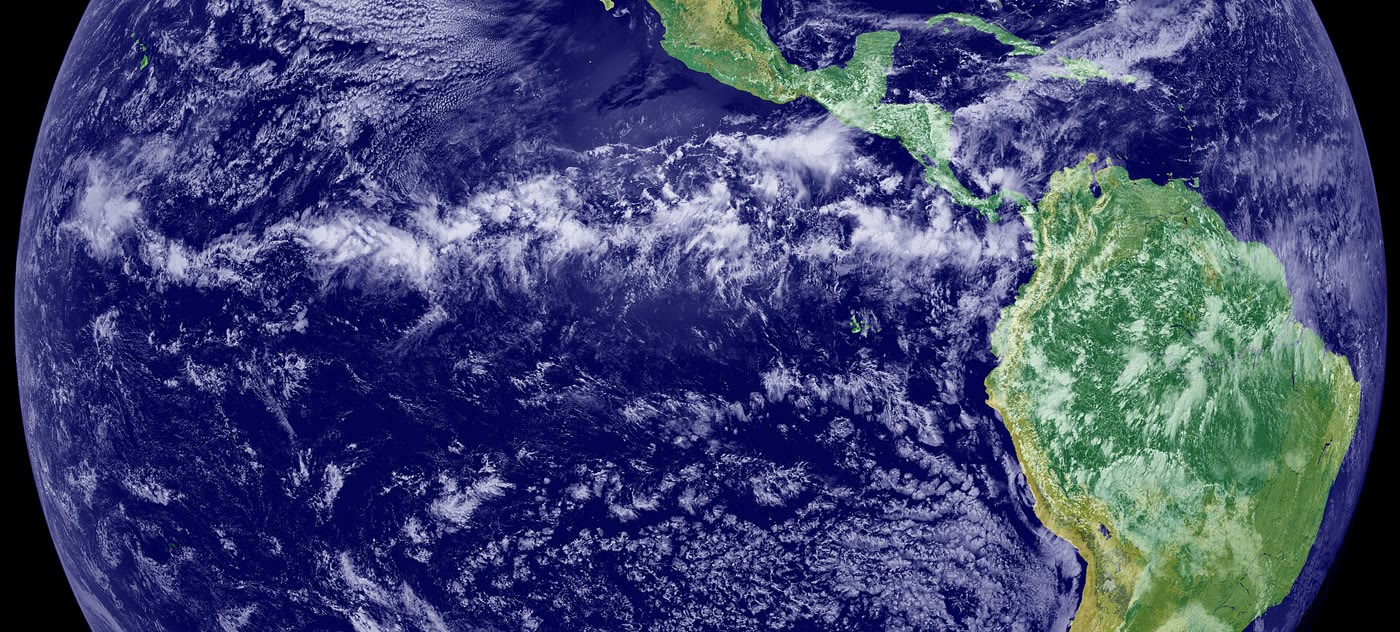
\includegraphics[width=0.8\linewidth]{images/book3/b1-itcz-goes.jpg}

{\small \omterm{def:b1:atmospheric-circulation:itcz}{منطقة التقارب بين المدارين} فوق شرق المحيط الهادئ: خطّ من السحب الساطعة يعبر المحيط شمال خطّ الاستواء، وأمريكا الوسطى والجنوبية على اليمين. تجمع الصورة بيانات السحب من القمر الاصطناعي الثابت بالنسبة إلى الأرض GOES-11 مع ألوان غطاء الأرض. (NASA Earth Observatory, ملك عام، عبر Wikimedia Commons.)}
\label{fig:b1:atmospheric-circulation:itcz-photo}
\end{omfigure}
% ledger: commons:itcz-goes

الهواء المتقارب يجب أن يصعد، والهواء الرطب الصاعد يبني السحب: \omterm{def:b1:atmospheric-circulation:itcz}{فمنطقة التقارب بين المدارين} هي أكثر الأحزمة مطرًا على الكوكب، وموضعها يُتتبَّع بخطّ العرض الذي تبلغ عنده الهطولات الزونالية المتوسطة ذروتها. وتتبع المنطقة الشمس مع تأخّر. وفي التحليل المُعاد تنتقل الذروة من \ang{12.8} جنوبًا في فبراير إلى \ang{10.9} شمالًا في سبتمبر؛ وبمتوسط الشهور الاثني عشر تقع عند \ang{2.6} شمالًا. ويُخفي المتوسط الزونالي فروقًا كبيرة بين \omterm{def:b1:spherical-astronomy:geographic}{خطوط الطول}: فوق شرق المحيط الهادئ في الصورة يقع النطاق شمال خطّ الاستواء، والمتوسط الزونالي يُجمع هذه النطاقات مع غيرها التي تتأرجح أبعد مع الفصول.
% ledger: data:b3-ncep (computed in figdata/bachelor-1/general_circulation.py)

\begin{omfigure}
\begin{tikzpicture}
\begin{axis}[omrecord, width=0.7\linewidth, height=5.2cm, xmin=0.5, xmax=12.5, ymin=-16, ymax=16,
  xlabel={الشهر}, ylabel={خطّ العرض (\unit{\degree})}, xtick={1,...,12},
  xticklabels={J,F,M,A,M,J,J,A,S,O,N,D}, ytick={-15,-10,...,15}]
% figdata/bachelor-1/general_circulation.py; ledger: data:b3-ncep
\addplot[black!40, domain=0.5:12.5] {0};
\addplot[omThm, line width=1.1pt, mark=*, mark size=1.6pt] table[x=month, y=lat] {figdata/out/bachelor-1-general_circulation-itcz.dat};
\end{axis}
\end{tikzpicture}

{\small خطّ العرض للحدّ الأقصى للهطول الزونالي المتوسط، شهرًا بشهر، بين \ang{20} جنوبًا و\ang{20} شمالًا: تتحرّك \omterm{def:b1:atmospheric-circulation:itcz}{منطقة التقارب بين المدارين} شمالًا في الصيف الشمالي وجنوبًا في الصيف الجنوبي، بشهرين أو ثلاثة خلف الشمس.
متوسطات NCEP-NCAR Reanalysis~1، 1991--2020، البيانات من NOAA PSL.}
\label{fig:b1:atmospheric-circulation:itcz}
\end{omfigure}
% ledger: data:b3-ncep

على طول خطّ الاستواء نفسه، حيث $f = 0$، يتحرّك الهواء مباشرةً على طول تدرّج الضغط، وتظهر دورة شرق-غرب فوق المحيط الهادئ.

\begin{definition}[دورة واكر]\label{def:b1:atmospheric-circulation:walker}
\emph{دورة واكر}\index{دورة واكر} هي الخليّة الدورانية شرق-غرب للغلاف الجوي على طول المحيط الهادئ الاستوائي: يصعد الهواء فوق المياه الدافئة في الغرب، حول القارة البحرية، ويتدفّق شرقًا في الأعلى، ويهبط فوق شرق المحيط الهادئ ويعود غربًا قرب السطح مع \omterm{def:b1:atmospheric-circulation:winds}{الرياح التجارية}.
\end{definition}
% ledger: climategov:walker

\begin{omfigure}
\begin{tikzpicture}[>={Stealth[length=2mm]}, font=\scriptsize]
  \fill[blue!12] (0,0) rectangle (11,0.45);
  \shade[left color=orange!45, right color=blue!12] (0,0) rectangle (6,0.45);
  \fill[brown!45] (-0.9,0) rectangle (0,0.6);
  \fill[brown!45] (11,0) rectangle (11.9,0.6);
  \node[anchor=north] at (-0.45,-0.05) {البحرية};
  \node[anchor=north] at (-0.45,-0.35) {القارة};
  \node[anchor=north] at (11.45,-0.05) {أمريكا};
  \node[anchor=north] at (11.45,-0.35) {الجنوبية};
  \node[anchor=north] at (5.5,-0.05) {المحيط الهادئ الاستوائي};
  \node at (1.6,0.22) {مياه دافئة};
  \foreach \x in {0.6,1.2,1.8} \fill[black!20] (\x,2.6) circle (0.45);
  \foreach \x in {0.9,1.5} \fill[black!25] (\x,3.0) circle (0.4);
  \draw[line width=1.2pt, omThm, ->] (9.5,0.8) -- (2.0,0.8);
  \draw[line width=1.2pt, omThm, ->] (1.2,1.0) -- (1.2,3.0);
  \draw[line width=1.2pt, omThm, ->] (2.0,3.3) -- (9.5,3.3);
  \draw[line width=1.2pt, omThm, ->] (10.3,3.0) -- (10.3,1.0);
  \node[anchor=south] at (5.75,0.85) {الرياح التجارية، من الشرق إلى الغرب};
  \node[anchor=south] at (5.75,3.35) {تدفّق العودة في الأعلى، من الغرب إلى الشرق};
  \node[anchor=west, align=left] at (1.6,1.8) {هواء صاعد،\\مطر غزير};
  \node[anchor=east, align=right] at (10.0,1.8) {هواء هابط،\\جاف};
\end{tikzpicture}

{\small \omterm{def:b1:atmospheric-circulation:walker}{دورة واكر} على طول المحيط الهادئ الاستوائي (تخطيطي؛ الارتفاع غير مرسوم بمقياس): صعود فوق الغرب الدافئ، وتدفّق شرقًا في الأعلى، وهبوط في الشرق ورجوع غربًا قرب السطح مع \omterm{def:b1:atmospheric-circulation:winds}{الرياح التجارية}.}
\label{fig:b1:atmospheric-circulation:walker}
\end{omfigure}
% ledger: climategov:walker

تكون \omterm{def:b1:atmospheric-circulation:walker}{دورة واكر} غير ثابتة. فحين تضعف، يضعف الصعود فوق القارة البحرية، وقد يهبط الهواء هناك حتى؛ وحين تقوى، يزداد الصعود والمطر فوق الغرب. وهذه التأرجحات، أي إل نينيو ولا نينيا، والانعكاسات الفصلية للرياح الموسمية، موضوع المجلّد الثاني. وخلال العقود منذ 1980، يجد تقييم 2021 للهيئة الحكومية الدولية المعنية بتغيّر المناخ \emph{احتمالًا كبيرًا جدًّا} لتقوية \omterm{def:b1:atmospheric-circulation:walker}{دورة واكر}، تشبه حالة لا نينيا، وانزياحًا غربيًّا، مع \emph{ثقة متوسطة} في حجم التغيّرات.
% ledger: climategov:walker, ipcc:hadley-widening

\section{التيّارات النفّاثة}\label{sec:b1:atmospheric-circulation:jets}

\begin{definition}[التيّار النفّاث؛ التيّارات النفّاثة شبه المدارية وجبهة القطب]\label{def:b1:atmospheric-circulation:jet}
\emph{التيّار النفّاث}\index{التيّار النفّاث} نطاق ضيّق من ريح قوية، عادةً ريح أفقية مرتفعة في التروبوسفير، يتغيّر موضعها من يوم إلى آخر. ويهبّ \emph{التيّار النفّاث شبه المداري}\index{التيّار النفّاث شبه المداري} من الغرب قرب الحافّة نحو القطب \omterm{def:b1:atmospheric-circulation:cells}{لخليّة هادلي}، عادةً بين \ang{20} و\ang{30} من خطّ العرض، على ارتفاعات \qtyrange{12}{14}{km}. ويهبّ \emph{تيّار جبهة القطب}\index{تيّار جبهة القطب} من الغرب فوق الحدّ الفاصل بين الهواء القطبي والهواء شبه المداري، بين نحو \ang{50} و\ang{60}؛ وهو النواة السريعة للرياح الغربية، تتحكّم فيه المنخفضات والمرتفعات الجوّية في \omterm{def:b1:spherical-astronomy:geographic}{خطوط العرض} الوسطى وتتحكّم فيها.
\end{definition}
% ledger: nws:jets, noaajs:jet

تُوجد التيّارات النفّاثة عادةً قرب \qty{9}{km}، ويمكن أن تبلغ أكثر من \qty{440}{km/h}، وتكون أقوى في شتاء كل نصف كرة، حين يكون التباين الحراري بين المدارين والقطب أكبر ما يكون. \omterm{def:b1:atmospheric-circulation:jet}{والتيّار النفّاث شبه المداري} هو ريح الزخم الزاوي من \cref{prop:b1:atmospheric-circulation:angular-momentum}، مروَّضة بالدوّامات؛ وهو يقع على حافّة \omterm{def:b1:atmospheric-circulation:cells}{خليّة هادلي}، قرب \ang{30} في المتوسط الشتوي. أمّا \omterm{def:b1:atmospheric-circulation:jet}{تيّار جبهة القطب} فيتأرجح شمالًا وجنوبًا مع مرور المنخفضات، والمتوسط حول الكرة يمحوه؛ ففي المتوسط الزونالي للصيف الشمالي لا يبقى إلا ذروة ضعيفة قدرها \qty{21.6}{m/s} قرب \ang{42.5} شمالًا، وفي الصيف الجنوبي \qty{29.9}{m/s} قرب \ang{47.5} جنوبًا. ولماذا تزداد الريح مع الارتفاع حيث تهبط الحرارة نحو القطب، أي الريح الحرارية، فذلك يُعرض في المجلّد الخاص بالسنة الثالثة.
% ledger: noaajs:jet, nws:jets, data:b3-ncep-circ (computed in figdata/bachelor-1/general_circulation.py)

\section{التمارين}

\begin{exercise}[$\star$]\label{exo:b1:atmospheric-circulation:1}
خذ $\Omega = \qty{7.292e-5}{rad.s^{-1}}$. (أ)~احسب \omterm{def:b1:atmospheric-circulation:coriolis-parameter}{معامل كوريوليس} عند
\ang{0}، و\ang{30}، و\ang{45} و\ang{90} شمالًا. (ب)~احسب التسارع الأفقي لكوريوليس لريح قدرها \qty{10}{m/s} عند \ang{45} شمالًا، وقارنه ب$g =
\qty{9.81}{m.s^{-2}}$. (ج)~في أيّ اتجاه يشير إذا كانت الريح تهبّ نحو الشمال؟
% ledger: earth:Trot
\end{exercise}

\begin{exercise}[$\star$]\label{exo:b1:atmospheric-circulation:2}
خطّان متساويا الضغط يفصل بينهما \qty{4}{hPa} يبعدان \qty{400}{km} عند مستوى البحر، حيث $\rho =
\qty{1.225}{kg.m^{-3}}$. (أ)~احسب التسارع الناتج عن \omterm{def:b1:atmospheric-circulation:pgf}{قوة تدرّج الضغط}. (ب)~لو لم يؤثّر شيء آخر، كم يلزم لتسريع الهواء الساكن إلى \qty{10}{m/s}؟ (ج)~قارن هذا التسارع بتسارع كوريوليس لريح قدرها \qty{10}{m/s} عند \ang{45} شمالًا، وقل ما الذي يوحي به هذا.
% ledger: ussa76:sea-level, earth:Trot
\end{exercise}

\begin{exercise}[$\star$]\label{exo:b1:atmospheric-circulation:3}
عند \ang{40} شمالًا، خطّان متساويا الضغط يفصل بينهما \qty{4}{hPa} يبعدان \qty{250}{km}؛ خذ $\rho =
\qty{1.225}{kg.m^{-3}}$. (أ)~احسب \omterm{def:b1:atmospheric-circulation:geostrophic}{الريح الجيوستروفية} بوحدة \unit{m/s} وبالعُقد
(\qty{1}{kn} = \qty{0.5144}{m/s}). (ب)~المنخفض يقع جنوبًا. من أيّ اتجاه تهبّ الريح؟ (ج)~صِف ريش الريح (العصا والريش) الذي يرسمه المتنبّئ الجوّي.
% ledger: ussa76:sea-level, earth:Trot
\end{exercise}

\begin{exercise}[$\star$]\label{exo:b1:atmospheric-circulation:4}
تعطي المتوسطات السنوية للتحليل المُعاد، قرب الأرض، الريح الشرقية \qty{-3.5}{m/s} عند \ang{15} شمالًا، و\qty{-4.4}{m/s} عند \ang{15} جنوبًا، و\qty{+1.9}{m/s} عند
\ang{45} شمالًا و\qty{+6.5}{m/s} عند \ang{45} جنوبًا، وضغط مستوى البحر \qty{1011.8}{hPa} عند \ang{15} شمالًا، و\qty{1016.8}{hPa} عند \ang{30} شمالًا و
\qty{1015.8}{hPa} عند \ang{45} شمالًا. (أ)~سمِّ نطاق الرياح عند كل من الخطوط العرضية الأربعة. (ب)~فسّر إشارة كل ريح بالفرع السطحي لخليّة. (ج)~أين يقع \omterm{def:b1:atmospheric-circulation:cells}{المرتفع شبه المداري} في نصف الكرة الشمالي بحسب هذه الضغوط؟
% ledger: data:b3-ncep-circ
\end{exercise}

\begin{exercise}[$\star\star$]\label{exo:b1:atmospheric-circulation:5}
ينشأ تدرّج ضغط قدره \qty{2}{hPa} لكل \qty{500}{km}، مع $\rho =
\qty{1.225}{kg.m^{-3}}$، عند \ang{60} و\ang{50} و\ang{30} و\ang{20} و\ang{10} و\ang{5} شمالًا. (أ)~احسب \omterm{def:b1:atmospheric-circulation:geostrophic}{الريح الجيوستروفية} عند كل خطّ عرض. (ب)~نادرًا ما تتجاوز رياح المدارات العميقة بضعة أمتار في الثانية مع تدرّجات كهذه. فسّر لماذا يفشل \omterm{def:b1:atmospheric-circulation:geostrophic}{التوازن الجيوستروفي} قرب خطّ الاستواء، مستخدمًا الزمن $1/f$ الذي تحتاجه قوة كوريوليس لتدوير الريح.
% ledger: ussa76:sea-level, earth:Trot
\end{exercise}

\begin{exercise}[$\star\star$]\label{exo:b1:atmospheric-circulation:6}
(أ)~باستخدام \cref{prop:b1:atmospheric-circulation:angular-momentum}، احسب ريح حلقة هواء تغادر خطّ الاستواء ساكنة، عند \ang{10} و\ang{15} و\ang{20} و\ang{30}؛ خذ $\Omega a_\oplus = \qty{464.6}{m/s}$. (ب)~الشيء نفسه لحلقة تبدأ ساكنة عند \ang{10} و\ang{15} و\ang{20} و\ang{30}. (ج)~يمتدّ الفرع الصاعد \omterm{def:b1:atmospheric-circulation:cells}{لخليّة هادلي} على خطوط عرض بدلًا من أن يكون عند خطّ الاستواء بالضبط. كيف يغيّر هذا \omterm{def:b1:atmospheric-circulation:jet}{التيّار النفّاث} المتوقّع؟
% ledger: earth:Trot, earth:Rmean
\end{exercise}

\begin{exercise}[$\star\star$]\label{exo:b1:atmospheric-circulation:7}
(أ)~سفينة في نصف الكرة الشمالي ترى الريح من الجنوب الغربي. باستخدام قانون بايس بالوت، أين مركز الضغط المنخفض؟ (ب)~سفينة في نصف الكرة الجنوبي ترى الريح من الشمال الغربي. أين المنخفض؟ (ج)~قرب الأرض تعبر الريح الخطوط المتساوية الضغط نحو الضغط المنخفض. هل يغيّر هذا إجابتك عن (أ) بتدوير اتجاه المنخفض في عقارب الساعة أو عكسها؟
% ledger: skybrary:buys-ballot
\end{exercise}

\begin{exercise}[$\star\star$]\label{exo:b1:atmospheric-circulation:8}
(أ)~احسب كتلة الهواء بين خطّ الاستواء و\ang{30} شمالًا، وبين مستويي الضغط \qty{1000}{hPa} و\qty{100}{hPa}، مع $a_\oplus = \qty{6371}{km}$
و$g = \qty{9.81}{m.s^{-2}}$. (ب)~في المتوسط السنوي، تحمل \omterm{def:b1:atmospheric-circulation:cells}{خليّة هادلي} الشمالية في التحليل المُعاد \qty{8.7e10}{kg/s}. كم يلزم لتمرير تلك الكتلة عبر الخليّة مرّة؟ (ج)~السؤال نفسه مع خليّة الشتاء الشمالي، \qty{21.4e10}{kg/s}.
% ledger: earth:Rmean, data:b3-ncep-circ
\end{exercise}

\begin{exercise}[$\star\star$]\label{exo:b1:atmospheric-circulation:9}
افترض أنه تحت مرتفع شبه مداري يهبط الهواء بسرعة \qty{1}{cm/s}، وأنه غير مشبع. (أ)~كم يهبط في يوم؟ (ب)~كم يسخن في يوم، إن لم يؤثّر شيء آخر، \omterm{def:b1:fluid-envelopes-structure:lapse-rate}{بمعدّل الانخفاض الأديباتي الجاف} \qty{9.8}{K/km}؟ (ج)~لا يسخن الهواء بهذا القدر يومًا بعد يوم. أيّ عملية من \cref{ch:b1:radiation-heat-transport} توازن الاحترار؟ (د)~لماذا تقع كثير من الصحاري الحارّة الكبرى تحت هذه المرتفعات؟
% ledger: nws:dalr
\end{exercise}

\begin{exercise}[$\star\star\star$]\label{exo:b1:atmospheric-circulation:10}
عند \ang{50} شمالًا، خذ $f = \qty{1.117e-4}{s^{-1}}$ وخطوطًا متساوية الضغط دائرية نصف قطرها $r = \qty{500}{km}$ (\cref{rem:b1:atmospheric-circulation:gradient}). (أ)~حول منخفض تبلغ فيه \omterm{def:b1:atmospheric-circulation:geostrophic}{الريح الجيوستروفية} \qty{15}{m/s}، حُلّ $V^2/r + fV =
f|\vec v_g|$ من أجل ريح التدرّج $V$. (ب)~حول مرتفع، بيّن أن $V^2/r - fV + f
|\vec v_g| = 0$ لا يملك حلًّا إلا إذا كان $|\vec v_g| \leq fr/4$، واحسب ذلك الحدّ. (ج)~ماذا يعني (ب) لتباعد الخطوط المتساوية الضغط قرب مركز \omterm{def:b1:atmospheric-circulation:cyclone}{المرتفع الجوّي}، مقارنةً بالمنخفض؟
\end{exercise}

\begin{exercise}[$\star\star\star$]\label{exo:b1:atmospheric-circulation:11}
(أ)~بيّن أنه ل$\varphi$ صغيرة (بالراديان) تكون ريح حلقة تغادر خطّ الاستواء ساكنة $u \approx \Omega a_\oplus\varphi^2$. (ب)~قارن التقريب بالصيغة الدقيقة عند \ang{10}، مع $\Omega a_\oplus = \qty{464.6}{m/s}$. (ج)~تبلغ الريح الزونالية المتوسطة السنوية للتحليل المُعاد عند \qty{200}{hPa} ذروتها \qty{27.0}{m/s} قرب \ang{35} شمالًا. عند أيّ خطّ عرض تبلغ الحلقة هذه السرعة؟ (د)~ماذا تقول الإجابة عن مدى الوثوق بحجّة الزخم الزاوي؟
% ledger: earth:Trot, earth:Rmean, data:b3-ncep-circ
\end{exercise}

\begin{exercise}[$\star\star\star$]\label{exo:b1:atmospheric-circulation:12}
تبلغ ذروة الهطول الزونالي المتوسط للتحليل المُعاد عند \omterm{def:b1:spherical-astronomy:geographic}{خطوط العرض} التالية، من يناير إلى ديسمبر: \ang{-10.5}، و\ang{-12.8}، و\ang{-5.8}، و\ang{-4.6}، و\ang{5.5}، و\ang{7.3}، و\ang{8.6}، و\ang{10.4}، و\ang{10.9}، و\ang{9.1}، و\ang{7.4}، و\ang{6.2}
(السالب: جنوبًا). (أ)~احسب المتوسط السنوي والمدى. (ب)~يبلغ خطّ العرض الشمسي تحت الشمس أقصاه في يونيو وديسمبر. بكم شهرًا تتأخّر \omterm{def:b1:atmospheric-circulation:itcz}{منطقة التقارب بين المدارين} عنه، وما الذي في النظام المناخي يستطيع أن يخزّن الحرارة فيُحدث مثل هذا التأخّر؟ (ج)~افترض أنه فوق محيط واحد تبقى منطقة التقارب شمال خطّ الاستواء طوال السنة. فسّر كيف يمكن للمتوسط الزونالي مع ذلك أن يعبر خطّ الاستواء.
% ledger: data:b3-ncep
\end{exercise}

\section{مسألة: قراءة خريطة جوّية في خطوط العرض الوسطى}

\begin{problem}[{مسألة نهاية الأسبوع --- الريح عند محطة قرب \ang{50} شمالًا}]
\label{pb:b1:atmospheric-circulation:1}
% values: calc/ch28.py (invented map; jet from data:b3-ncep-circ)
تُظهر خريطة جوّية لشمال الأطلسي، قرب المحطة P عند \ang{50} شمالًا، خطوطًا متساوية الضغط مستقيمة تمتدّ من الغرب إلى الشرق، كل \qty{4}{hPa}، والضغوط الأخفض شمالًا. تقع P بين الخطّين \qty{1004}{hPa} و\qty{1008}{hPa}، وهما يبعدان \qty{250}{km} هناك؛ وضغطها عند مستوى البحر \qty{1006}{hPa}، وحرارة هوائها \qty{10}{\degreeCelsius}. الخريطة مخترعة، لكن أرقامها نموذجية. استخدم $\Omega = 2\pi/(\qty{23.9345}{h})$، و$a_\oplus = \qty{6371}{km}$، و$R_d =
\qty{287.05}{J.kg^{-1}.K^{-1}}$ للهواء الجاف، و\qty{1}{kn} = \qty{0.514444}{m/s}.

\medskip
\noindent\textbf{الجزء الأول --- تدرّج الضغط \omterm{def:b1:atmospheric-circulation:geostrophic}{والريح الجيوستروفية}.}
\begin{enumerate}
  \item احسب كثافة الهواء عند P بقانون الغاز المثالي.
  \item احسب التدرّج الأفقي للضغط عند P، بوحدة \unit{Pa.m^{-1}}.
  \item احسب التسارع الناتج عن \omterm{def:b1:atmospheric-circulation:pgf}{قوة تدرّج الضغط}.
  \item احسب $\Omega$ \omterm{def:b1:atmospheric-circulation:coriolis-parameter}{ومعامل كوريوليس} عند \ang{50} شمالًا.
  \item احسب سرعة \omterm{def:b1:atmospheric-circulation:geostrophic}{الريح الجيوستروفية} عند P.
  \item عبّر عنها بالعُقد وبوحدة \unit{km/h}.
  \item بيّن أن الزمن الذي تحتاجه \omterm{def:b1:atmospheric-circulation:pgf}{قوة تدرّج الضغط} وحدها لتبلغ بالهواء الساكن سرعة الجيوستروفية هو $1/f$، واحسبه، مع الزمن $2\pi/f$ الذي تستغرقه قوة كوريوليس لتدوير الريح دورة كاملة.
\end{enumerate}

\medskip
\noindent\textbf{الجزء الثاني --- الاتجاه ونصف الكرة.}
\begin{enumerate}[resume]
  \item في أيّ اتجاه تشير \omterm{def:b1:atmospheric-circulation:pgf}{قوة تدرّج الضغط} عند P؟ وفي أيّ اتجاه تهبّ \omterm{def:b1:atmospheric-circulation:geostrophic}{الريح الجيوستروفية}، ومن أيّ سمت تأتي؟
  \item تحقّق من إجابتك بقانون بايس بالوت.
  \item صِف ريش الريح المرسوم عند P: اتجاه العصا، وعدد الريش، والجانب الذي تقف عليه.
  \item افترض أن الخطوط المتساوية الضغط نفسها، مع المنخفض شمالًا، وُجدت عند \ang{50} جنوبًا. من أيّ اتجاه تهبّ الريح؟
  \item مع الكثافة وتدرّج الضغط نفسيهما، احسب \omterm{def:b1:atmospheric-circulation:geostrophic}{الريح الجيوستروفية} عند \ang{30} شمالًا و\ang{60} شمالًا.
  \item احسبها عند \ang{5} شمالًا. هل النتيجة معقولة؟ فسّر.
\end{enumerate}

\medskip
\noindent\textbf{الجزء الثالث --- الريح عند الأرض.} يقيس مقياس الريح عند P ريحًا قدرها \qty{9.0}{m/s} تعبر الخطوط المتساوية الضغط بزاوية \ang{25} نحو الضغط المنخفض.
\begin{enumerate}[resume]
  \item احسب نسبة الريح المرصودة إلى \omterm{def:b1:atmospheric-circulation:geostrophic}{الريح الجيوستروفية}، ومركّبتي الريح المرصودة على طول الخطوط المتساوية الضغط وعبرها.
  \item من أيّ سمت تهبّ الريح المرصودة؟
  \item في نموذج الاحتكاك الخطّي ل\cref{prop:b1:atmospheric-circulation:friction}، أيّ ثابت زمني $\tau$ يعطي الزاوية المرصودة، وأيّ سرعة يتنبّأ بها النموذج عندئذٍ؟ قارنها بالرصد.
  \item حول منخفض نصف قطره \qty{500}{km}، افترض أن هواء الكيلومتر الأدنى يتدفّق نحو الداخل في كل مكان بالمركّبة العابرة للخطوط المتساوية الضغط في سؤال~14، وبكثافة السؤال~1. احسب كتلة الهواء الداخلة إلى المنخفض في الثانية.
  \item يجب أن يخرج هذا الهواء من أعلى الطبقة. احسب متوسط السرعة الرأسية الصاعدة هناك، بوحدة \unit{m/s} وبالأمتار في اليوم.
  \item عند \omterm{def:b1:fluid-envelopes-structure:lapse-rate}{معدّل الانخفاض الأديباتي الجاف} \qty{9.8}{K/km}، بكم يبرد الهواء الصاعد في يوم؟ ما الطقس الذي يتبع ذلك، وماذا كان سيحدث تحت مرتفع جوّي بدلًا من ذلك؟
\end{enumerate}

\medskip
\noindent\textbf{الجزء الرابع --- \omterm{def:b1:atmospheric-circulation:jet}{التيّار النفّاث} فوقه.} تبلغ الريح الزونالية المتوسطة عند \qty{200}{hPa} في الشتاء الشمالي ذروتها \qty{42.3}{m/s} قرب \ang{30} شمالًا (متوسطات التحليل المُعاد 1991--2020).
\begin{enumerate}[resume]
  \item احسب السرعة الشرقية للأرض عند خطّ الاستواء وعند \ang{30} شمالًا.
  \item تغادر حلقة هواء خطّ الاستواء ساكنة في الأعلى وتحتفظ بزخمها الزاوي. احسب ريحها عند \ang{20} شمالًا و\ang{30} شمالًا.
  \item السؤال نفسه عند \ang{30} شمالًا لحلقة تبدأ ساكنة عند \ang{10} شمالًا.
  \item بكم تتفوّق حلقة السؤال~21 على \omterm{def:b1:atmospheric-circulation:jet}{التيّار النفّاث} المرصود عند \ang{30} شمالًا؟ اعطِ سببين لكون التيّار الحقيقي أبطأ.
  \item احسب نسبة الزخم الزاوي المطلق لكل وحدة كتلة للتيّار النفّاث المرصود عند \ang{30} شمالًا إلى زخم الهواء الساكن عند خطّ الاستواء. ما الكسر الذي فُقد في الطريق؟
  \item ما سرعة \omterm{def:b1:atmospheric-circulation:geostrophic}{الريح الجيوستروفية} عند P، بالأمتار في الثانية، وكيف تُقارن بها الريح المقاسة عند الأرض؟
\end{enumerate}
\end{problem}
